\section{Objetivos}
\begin{itemize}
    \item Medir el torque magnético que se presenta en espiras con corriente ubicadas en un campo magnético y realizar el análisis de todos sus parámetros.
    \item Identificar la presencia de campos magnéticos con ayuda de una brújula.
    \item Definir la orientación del campo magnético producido por bobinas que llevan corriente.
\end{itemize}

\section{Marco Teórico}
La interacción de los campos magnéticos con conductores por los cuales circula corriente es fundamental en la comprensión y aplicación de numerosas tecnologías. Si un conductor por el cual fluye corriente se encuentra dentro de un campo magnético, experimentará una fuerza que es perpendicular tanto a la dirección del campo como al movimiento de la corriente.

\subsection{Fuerza sobre un Conductor en un Campo Magnético}
Cuando cargas eléctricas se mueven dentro de un campo magnético, experimentan una fuerza magnética descrita por la ley de Lorentz, que es proporcional al vector velocidad de las cargas, la intensidad del campo magnético y el seno del ángulo entre ellos. Esta fuerza es la base para el funcionamiento del motor eléctrico y otros dispositivos electromagnéticos.

\subsection{Momento de Torque sobre una Espira de Corriente}
Una espira de corriente dentro de un campo magnético experimenta un momento de torque, el cual tiende a alinear el plano de la espira con el campo magnético. Este torque es proporcional al área de la espira, la corriente, la intensidad del campo magnético y el seno del ángulo entre el plano de la espira y la dirección del campo.

\subsection{Bobinas de Helmholtz}
Las bobinas de Helmholtz se utilizan para crear campos magnéticos uniformes. Consisten en dos bobinas coaxiales separadas por una distancia igual al radio de las bobinas, que cuando son alimentadas con corriente, generan un campo magnético en la región entre ellas. Esta configuración permite estudios detallados del comportamiento de materiales y dispositivos en presencia de un campo magnético conocido y controlable.

\subsection{Campo Magnético Terrestre}
El campo magnético de la Tierra influye en muchos fenómenos naturales y tecnológicos. En el contexto de este laboratorio, actúa como un campo adicional que interactúa con los campos generados por dispositivos experimentales, como las bobinas de Helmholtz, y puede afectar las mediciones si no se toma en cuenta adecuadamente.

\section{Análisis y discusión: Montaje 1 Corriente fija en bobina $= 2.5A$}

\subsection{Ajustar la corriente}
\textbf{Ajustar la corriente I (de las bobinas de Helmholtz) a 2A. Con los parámetros fijados y
con la expresión de Helmholtz (5), calcular la intensidad del campo magnético.}

\begin{figure}[H]
  \centering
  \begin{subfigure}[b]{\textwidth}
      \centering
      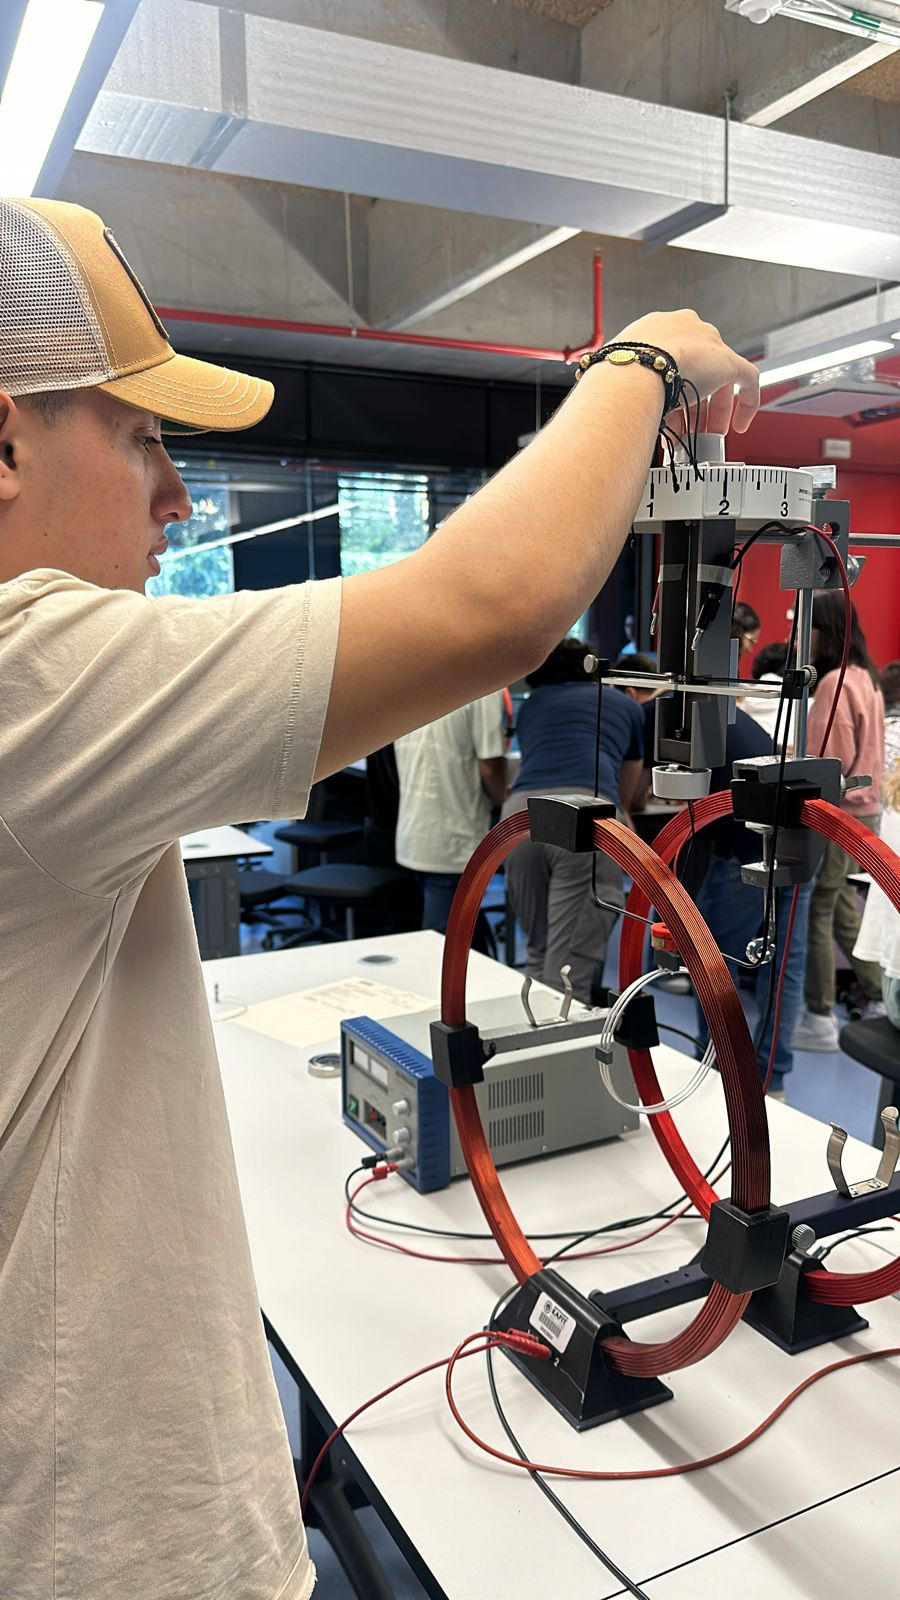
\includegraphics[width=0.4\textwidth]{Figures/1. Content/montaje.jpeg}
      \caption{Montaje de bobinas de Helmholtz}
      \label{fig: Montaje 1}
  \end{subfigure}
  \hfill
\end{figure}

\subsection{Colocar balanza de torsión}
\textbf{Coloque en la balanza de torsión una bobina de prueba de $N_3 = 3$ espiras, de tal
forma tal que el ángulo entre el campo magnético y la normal a la bobina de prueba
sea $\Theta = 90^{\circ}$. Con las dos fuentes apagadas, ajustar la posición de la balanza de
torsión en cero.}

\subsubsection{Encender fuentes}
\textbf{Encienda y ajuste las fuentes para que circule una corriente $i = 0.5A$ por la
bobina de prueba de tres vueltas y establecer $I=2.5A$ por las bobinas de
Helmohltz.}
\subsubsection{Equilibrar la balanza}
\textbf{Vuelva a equilibrar la balanza, mida y reporte este desplazamiento; esto es,
la fuerza aplicada en el brazo del dinamómetro $\tau E = F \times d$, donde $d=0.11m$ y $F$ es la lectura del dinamómetro (en miliNewtons).}

\subsubsection{Tabla de valores}
\textbf{Repita los pasos anteriores con las corrientes que se muestran en la tabla
siguiente y reporte los valores requeridos:}

\begin{figure}[H]
  \centering
  \begin{subfigure}[b]{\textwidth}
      \centering
      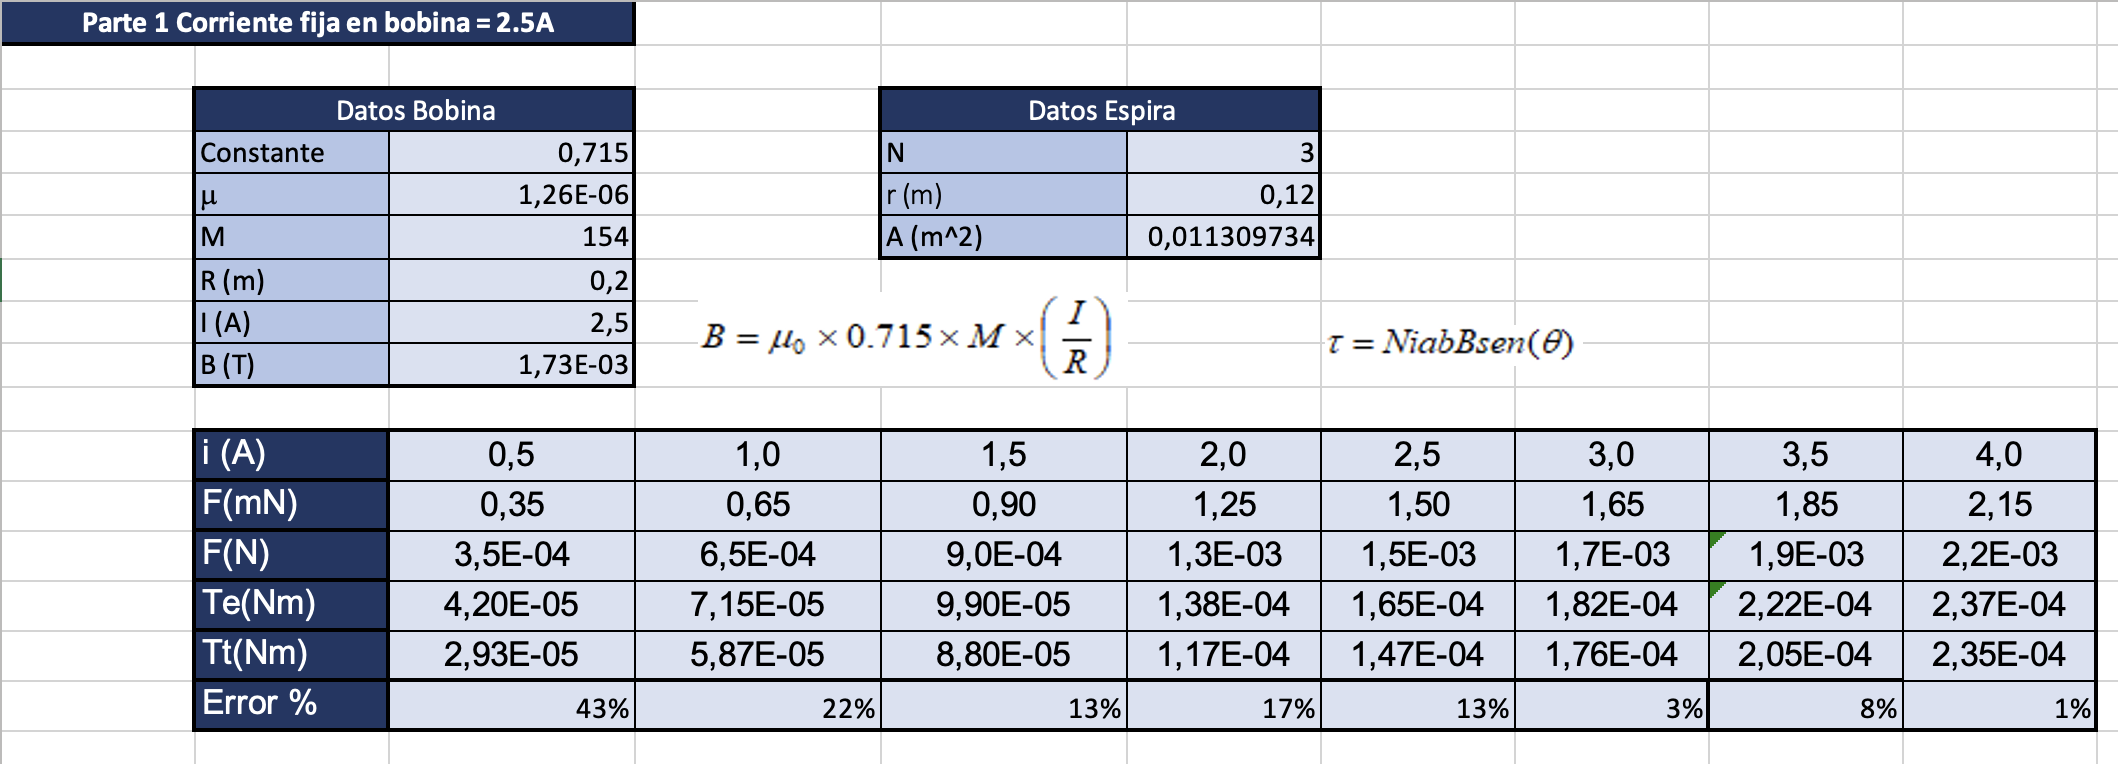
\includegraphics[width=\textwidth]{Figures/1. Content/tabla1.png}
      \caption{Tabla de Valores 1}
      \label{fig: Tabla 1}
  \end{subfigure}
  \hfill
\end{figure}

\subsubsection{$\tau$ vs $i$}
\textbf{Grafique $\tau$ vs $i$, teórico y práctico en un mismo plano cartesiano y
encontrar la pendiente. Describa el significado físico de esta pendiente.}

\begin{figure}[H]
  \centering
  \begin{subfigure}[b]{\textwidth}
      \centering
      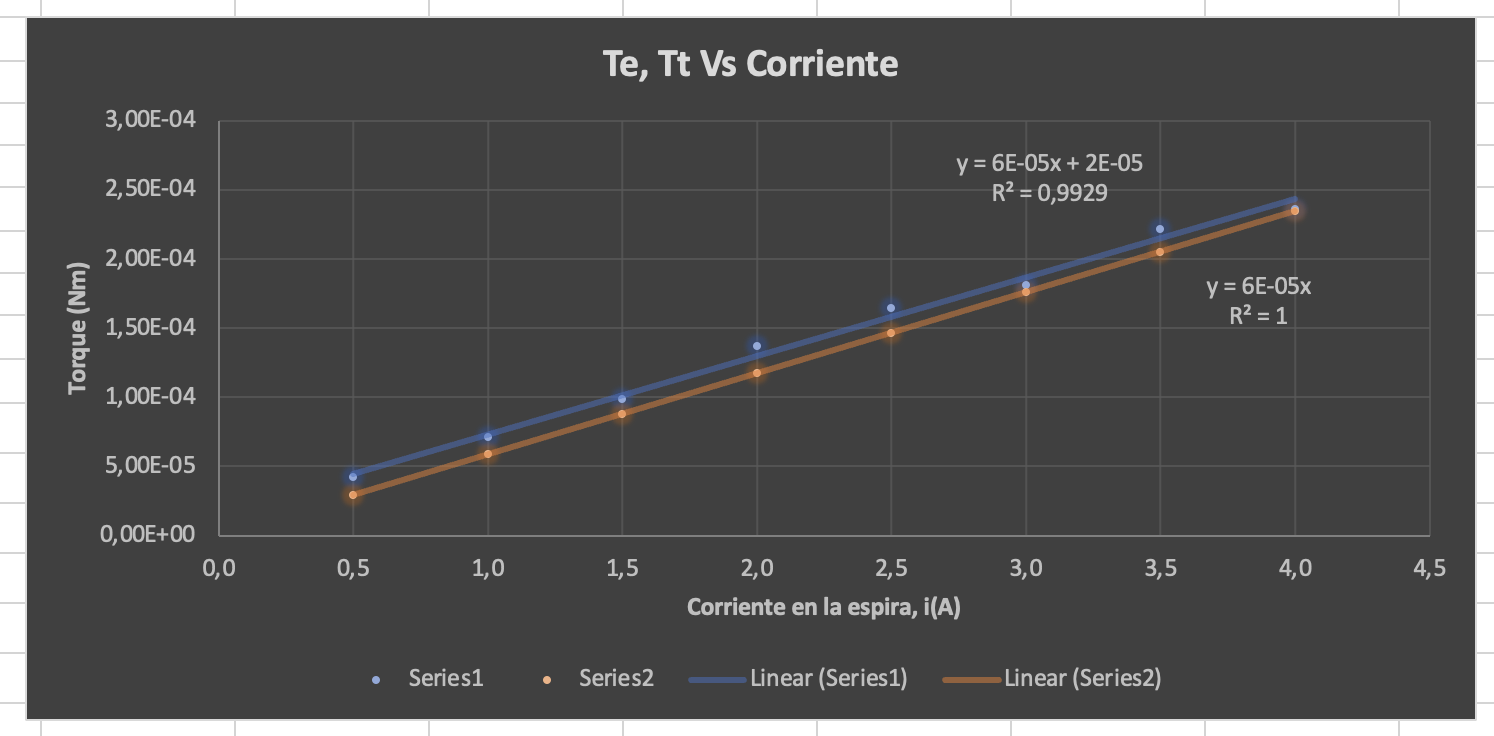
\includegraphics[width=\textwidth]{Figures/1. Content/grafica1.png}
      \caption{Gráfica de $\tau$ vs $i$ teórico y práctico. La pendiente representa la eficacia de la espira para convertir corriente eléctrica en torque mecánico bajo un campo magnético constante.}
      \label{fig: Grafica 1}
  \end{subfigure}
  \hfill
\end{figure}

En esta gráfica, las pendientes representan el cambio en el torque por unidad de cambio en la corriente, indican la relación proporcional entre estas variables, conforme a la ley física que describe cómo el torque en una espira es directamente proporcional a la corriente que fluye a través de ella en un campo magnético constante. Este análisis es crucial para entender la efectividad de la espira en convertir la energía eléctrica en mecánica.

\section{Análisis y discusión: Montaje 2 Corriente fija en espira $i = 3A$ Corriente en bobina cambiante}
\textbf{Utilice los siguientes parámetros: $i = 2.5A$, $N_3 = 3$, $\Theta = 90^{\circ}$. Apague las fuentes y
ajuste la balanza a su posición de cero}
\subsection{Tabla de valores}
\textbf{Varíe la corriente $I$ de acuerdo a los valores de la siguiente tabla:}

\begin{figure}[H]
  \centering
  \begin{subfigure}[b]{\textwidth}
      \centering
      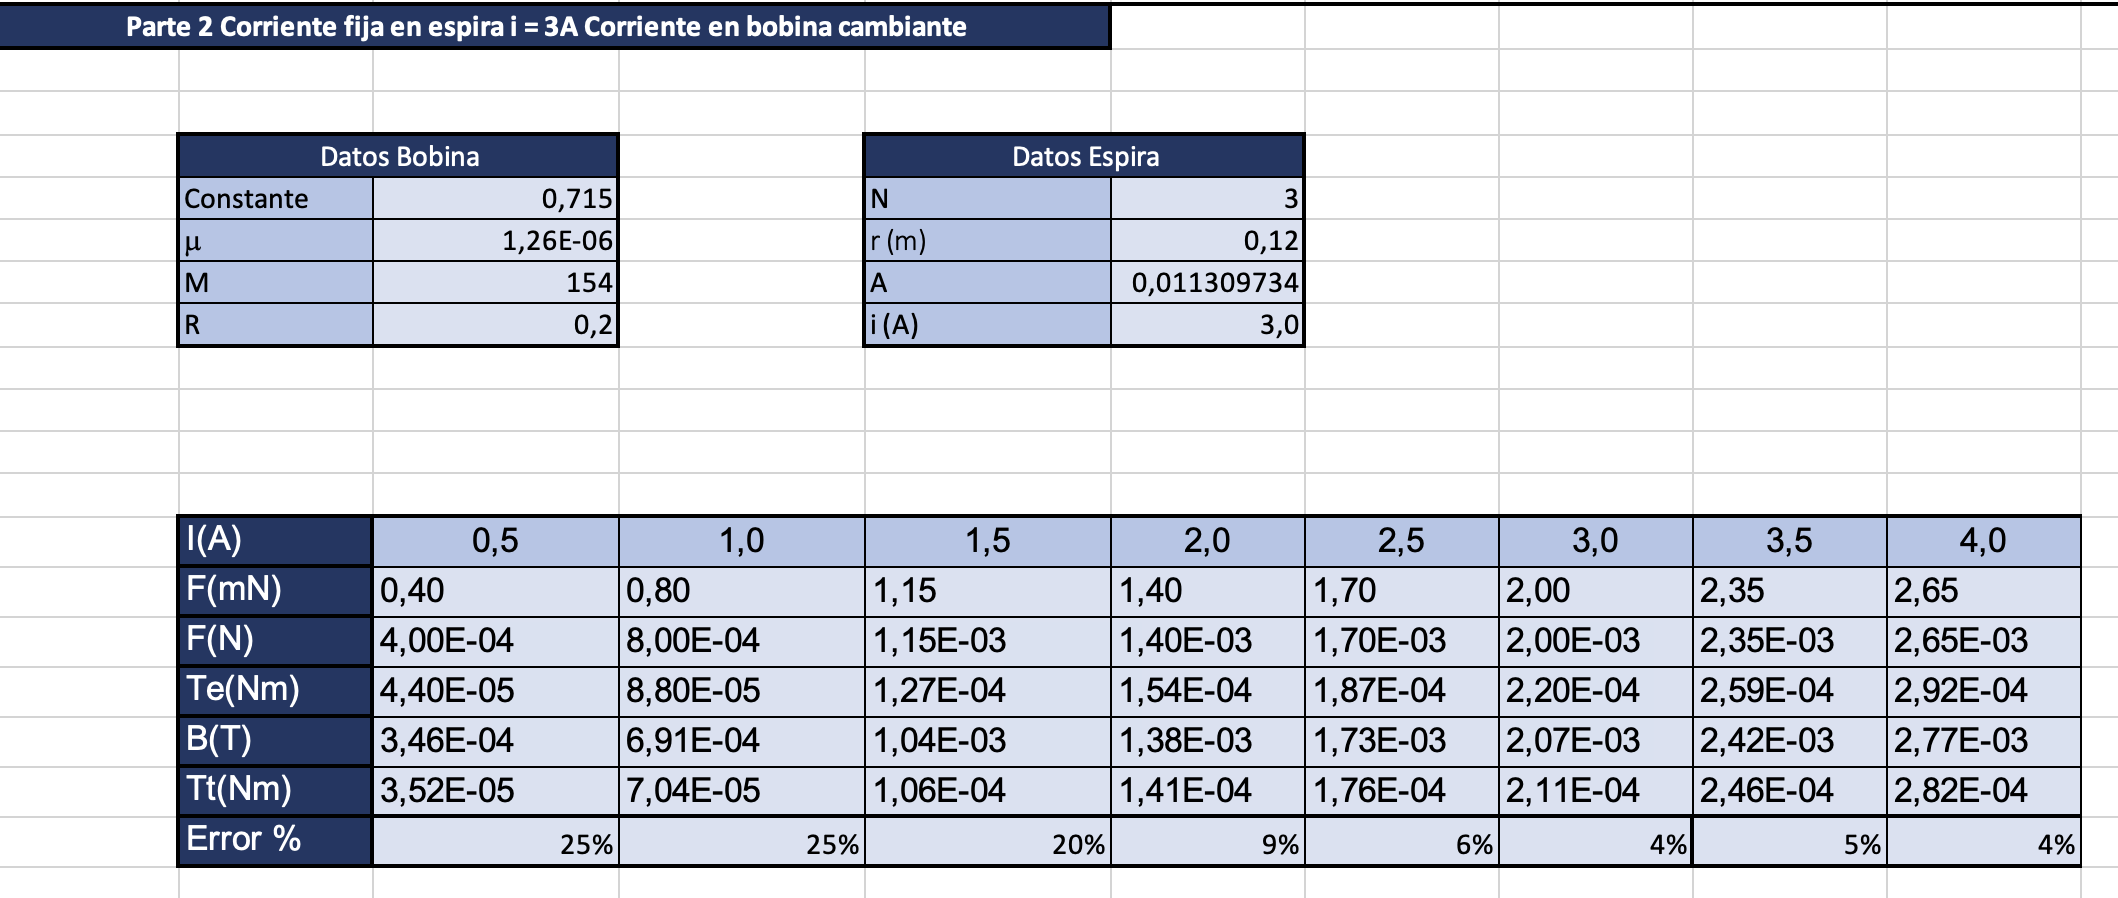
\includegraphics[width=\textwidth]{Figures/1. Content/tabla2.png}
      \caption{Tabla de Valores 2}
      \label{fig: Tabla 2}
  \end{subfigure}
  \hfill
\end{figure}

\subsection{$\tau$ vs $B$}
\textbf{Calcule el campo magnético $B$ con cada valor de corriente y grafique $\tau$ vs $B$, tanto
teórica como experimentalmente en un mismo plano cartesiano y encuentre la
pendiente. Describa el significado físico de esta pendiente.}

\begin{figure}[H]
  \centering
  \begin{subfigure}[b]{\textwidth}
      \centering
      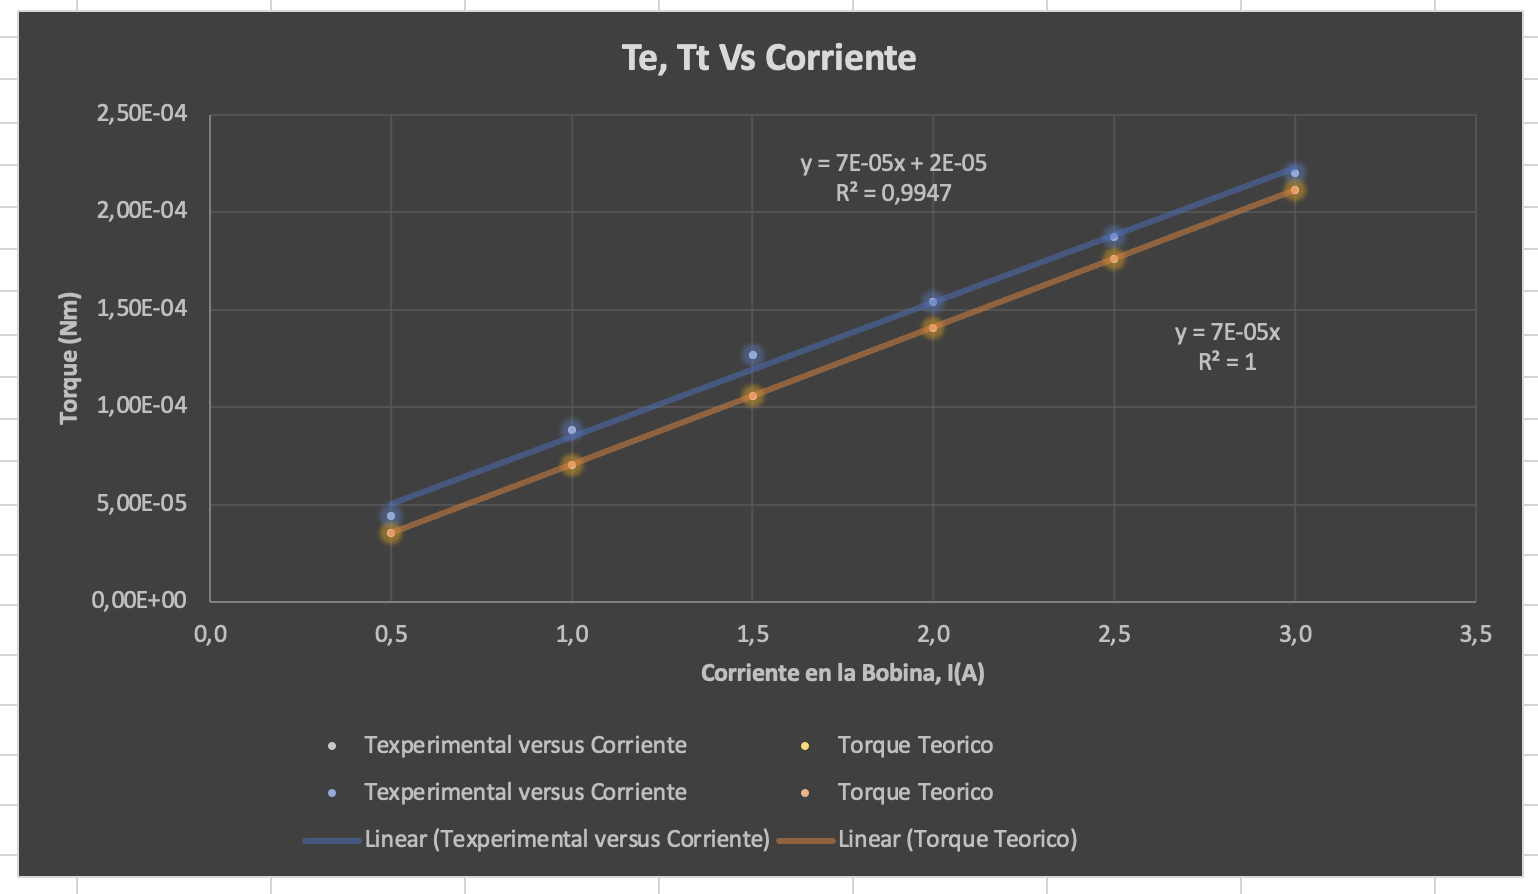
\includegraphics[width=\textwidth]{Figures/1. Content/grafica2.png}
      \caption{Gráfica $\tau$ vs $B$}
      \label{fig: Grafica 2}
  \end{subfigure}
  \hfill
\end{figure}

Analizando la pendiente de la gráfica $\tau$ vs $B$, y considerando la ecuación teórica para el torque en un campo magnético:

\[
\tau = N \cdot i \cdot A \cdot B \cdot \sin(\theta)
\]

donde $\sin(90^\circ) = 1$, simplificamos la expresión a:

\[
\tau = N \cdot i \cdot A \cdot B
\]

Dado que la gráfica se ajusta a una relación lineal descrita por la ecuación de la recta \(y = mx + b\), donde \(\tau = y\), \(B = x\) y la pendiente \(m = N \cdot i \cdot A\). Esto indica que la pendiente es igual a la multiplicación de los valores constantes del experimento: el número de espiras \(N\), la corriente \(i\) en la bobina de prueba y el área \(A\) de la espira. Así, la pendiente refleja cómo estos factores interactúan para influir en la magnitud del torque generado por el campo magnético aplicado, subrayando la relación proporcional directa entre el torque y el campo magnético para una configuración dada de la espira.

\section{Análisis y discusión: Montaje 3 Corriente fija en espira y bobina $i = 3A = I$ N Cambiante}
\textbf{Ajuste a los siguientes valores$I = i = 2A$ y $\Theta = 90^{\circ}$. Apague las fuentes y conecte
las bobinas de prueba de $3$, $2$, $1$ espiras de igual área y en cada caso realice las
medidas de torque.}
\subsection{Tabla de valores}
\textbf{Varíe la corriente $I$ de acuerdo a los valores de la siguiente tabla:}

\begin{figure}[H]
  \centering
  \begin{subfigure}[b]{\textwidth}
      \centering
      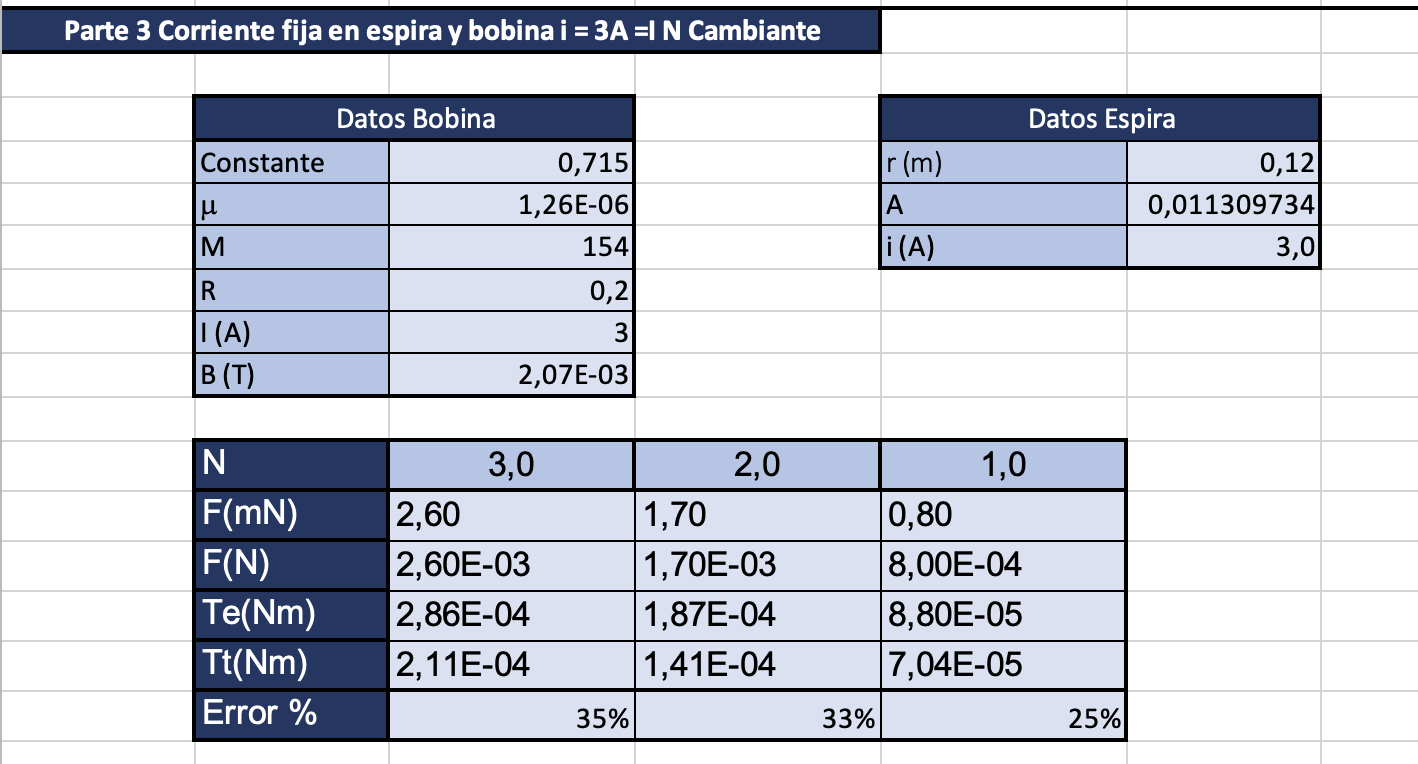
\includegraphics[width=\textwidth]{Figures/1. Content/tabla3.png}
      \caption{Tabla de Valores 3}
      \label{fig: Tabla 3}
  \end{subfigure}
  \hfill
\end{figure}

\subsection{$\tau$ vs $N$}
\textbf{Grafique $\tau$ vs $N$ teórico y práctico en un mismo plano cartesiano, obtenga la
pendiente y describa su significado físico.}

\begin{figure}[H]
  \centering
  \begin{subfigure}[b]{\textwidth}
      \centering
      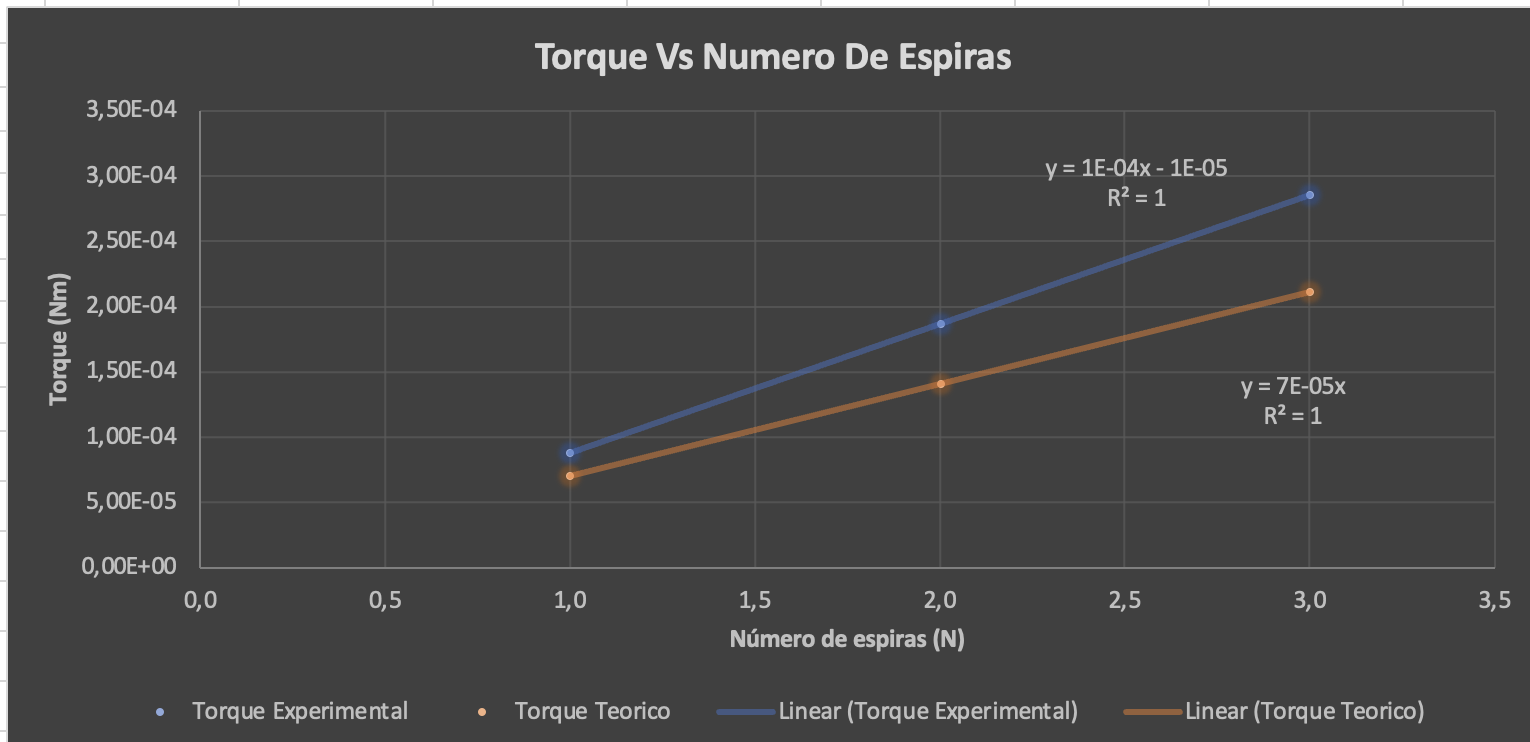
\includegraphics[width=\textwidth]{Figures/1. Content/grafica3.png}
      \caption{Gráfica $\tau$ vs $N$}
      \label{fig: Grafica 3}
  \end{subfigure}
  \hfill
\end{figure}

Al analizar la pendiente de la gráfica $\tau$ vs $N$ y considerar la ecuación teórica para el torque en un campo magnético:

\[
\tau = N \cdot i \cdot A \cdot B \cdot \sin(\theta)
\]

donde $\sin(90^\circ) = 1$, simplificamos esta a:

\[
\tau = N \cdot i \cdot A \cdot B
\]

Para esta relación, ajustada a la ecuación de la recta \(y = mx + b\), donde \(\tau = y\), \(N = x\) y \(m = i \cdot A \cdot B\). Esto significa que la pendiente es igual al producto de la corriente \(i\), el área \(A\) de la espira, y el campo magnético \(B\) producido por las bobinas de Helmholtz.

Esta pendiente indica que el torque es directamente proporcional al número de espiras \(N\) del conductor en el campo magnético. Cada espira adicional aumenta linealmente la fuerza magnética que experimenta el sistema, destacando la relación lineal entre el número de espiras y el torque generado en un campo magnético constante. Así, la pendiente proporciona una medida cuantitativa de cómo cada espira adicional contribuye al torque total ejercido sobre el sistema bajo las condiciones experimentales actuales.


\section{Análisis y discusión: Montaje 3 Corriente fija en espira $i = 3A = I = 3A$ Area Cambiante}
\textbf{Conecte bobinas de 1 espira y diferente área, en cada caso calcule el área y mida el
torque. Ajuste $I = i = 2A$, $N=1$, y $\Theta = 90^{\circ}$.}

\subsection{Tabla de valores}
\textbf{Varíe la corriente $I$ de acuerdo a los valores de la siguiente tabla:}

\begin{figure}[H]
  \centering
  \begin{subfigure}[b]{\textwidth}
      \centering
      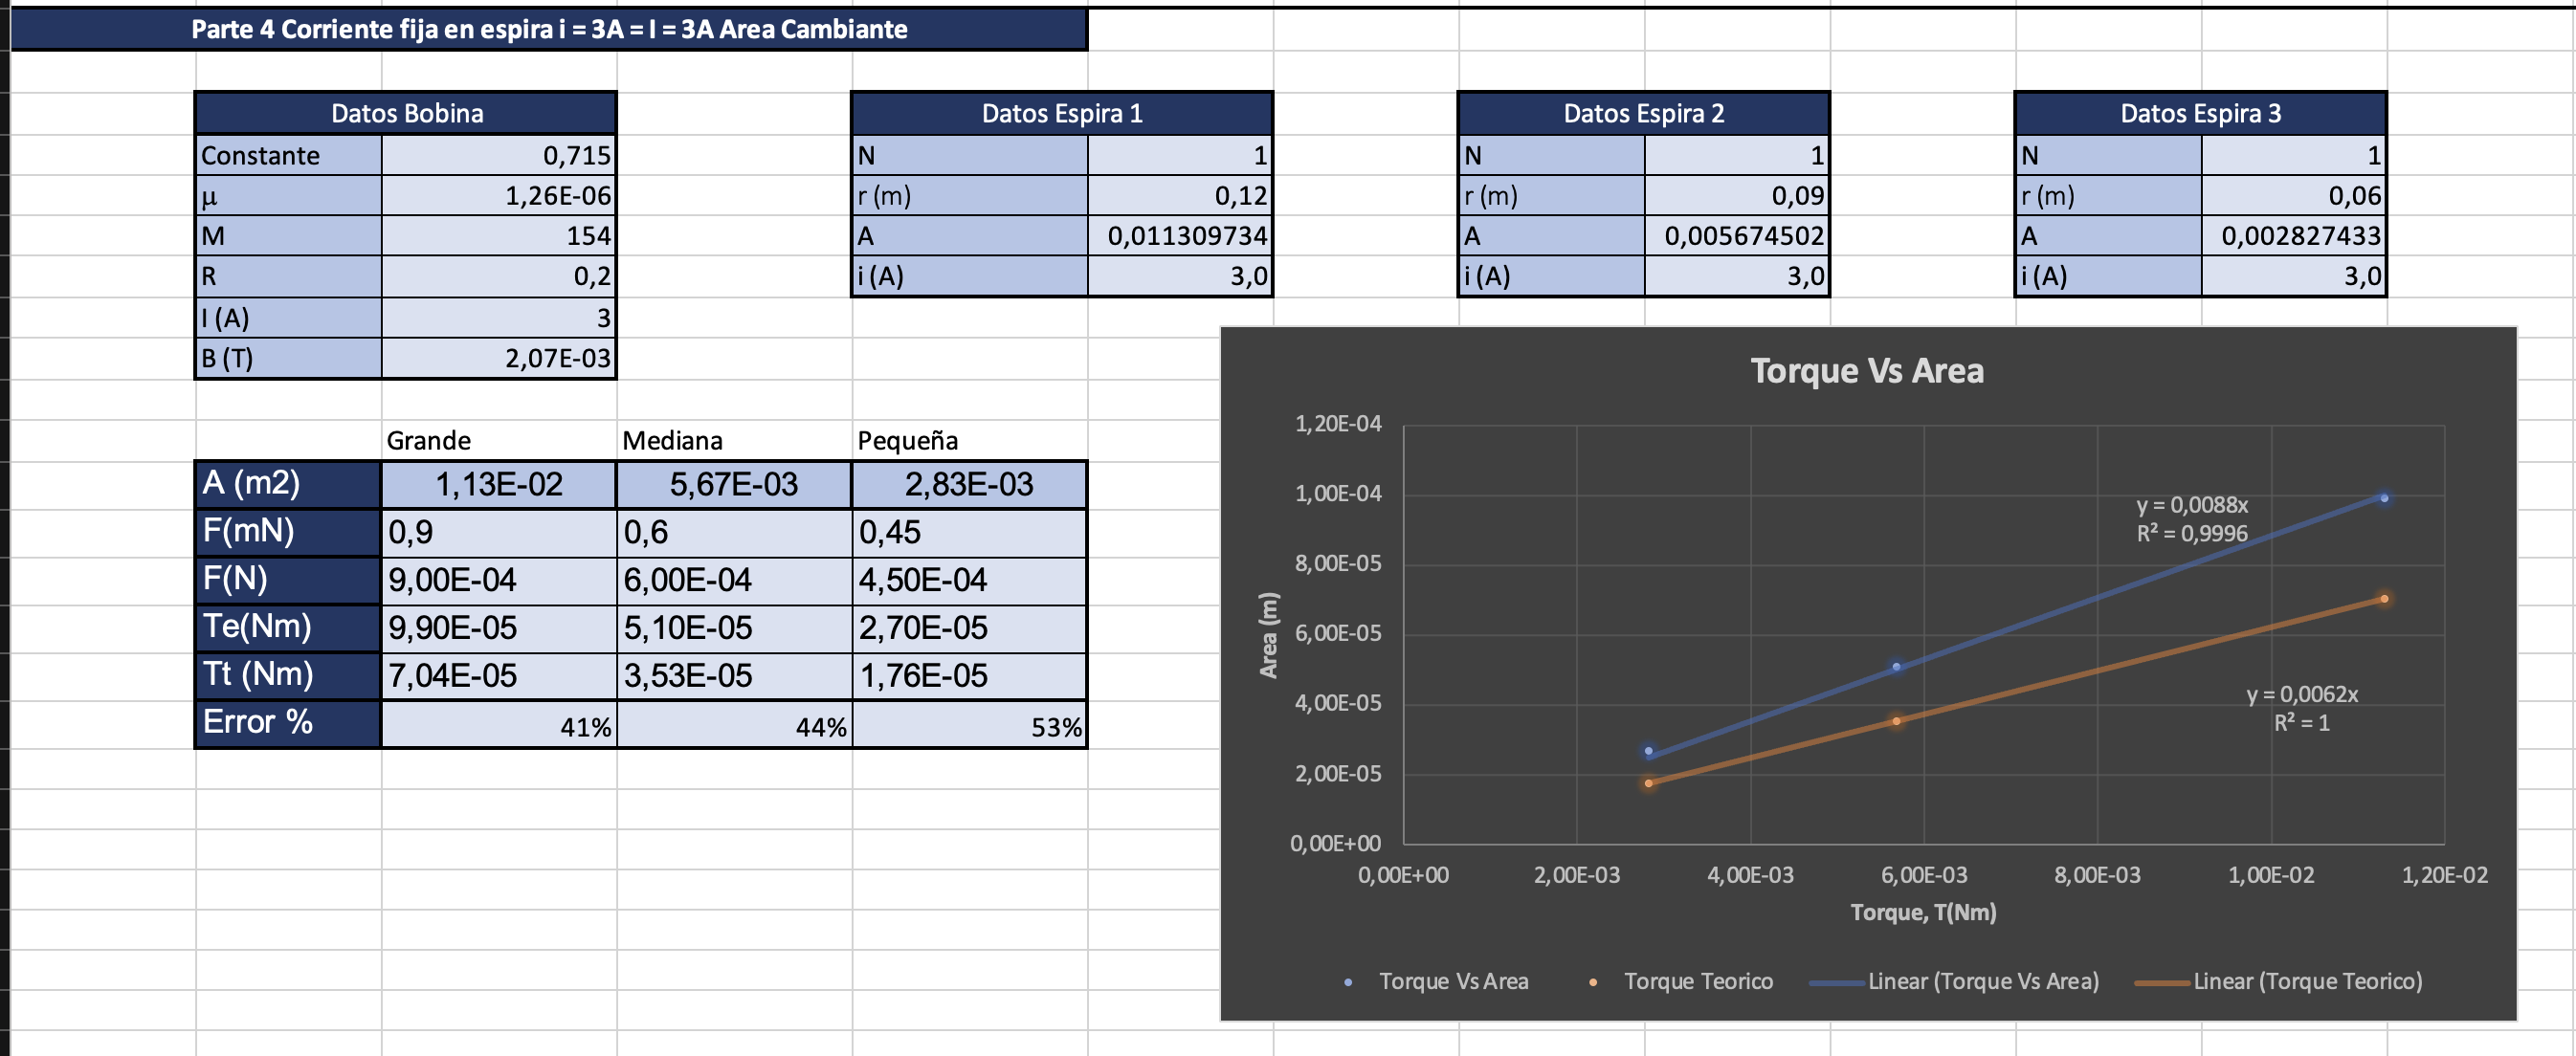
\includegraphics[width=\textwidth]{Figures/1. Content/tabla4.png}
      \caption{Tabla de Valores 4}
      \label{fig: Tabla 4}
  \end{subfigure}
  \hfill
\end{figure}

\subsection{$\tau$ vs $A$}
\textbf{Grafique $\tau$ vs $A$ , teórico y práctico sobre un mismo plano cartesiano, obtenga la
pendiente y describa su significado físico.}

\begin{figure}[H]
  \centering
  \begin{subfigure}[b]{\textwidth}
      \centering
      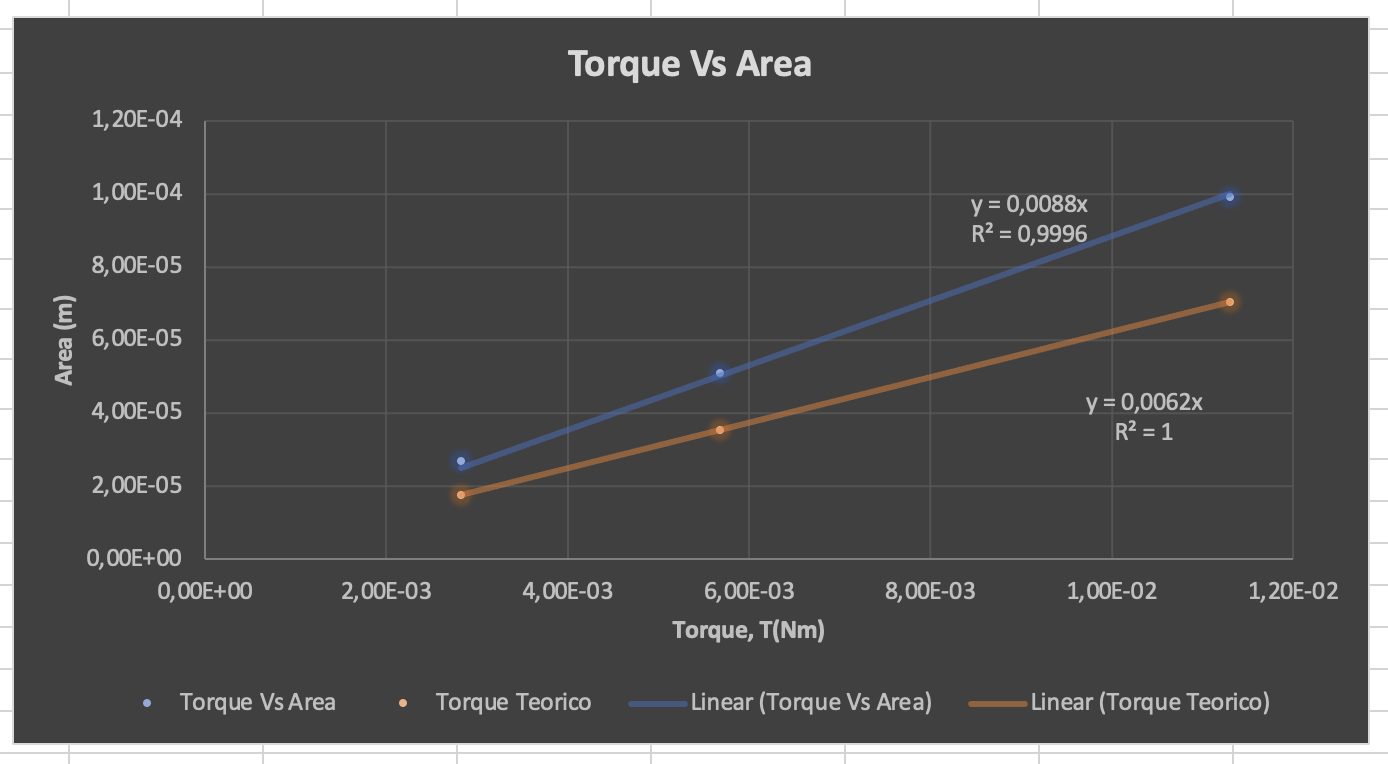
\includegraphics[width=\textwidth]{Figures/1. Content/grafica4.png}
      \caption{$\tau$ vs $A$}
      \label{fig: Grafica 4}
  \end{subfigure}
  \hfill
\end{figure}

El torque (\(\tau\)) ejercido sobre un conductor en un campo magnético se describe mediante la relación:
\[
\tau = N \cdot i \cdot A \cdot B \cdot \sin(\theta),
\]
donde \(N\) es el número de espiras, \(i\) la corriente a través del conductor, \(A\) el área del lazo del conductor, \(B\) la intensidad del campo magnético, y \(\theta\) el ángulo entre el campo y la normal al área del conductor. Suponiendo que \(\theta = 90^\circ\), \(\sin(\theta) = 1\), simplificando la ecuación a:
\[
\tau = N \cdot i \cdot A \cdot B.
\]

En esta configuración, la gráfica de \(\tau\) versus \(A\) teórica y experimental permite determinar cómo el torque varía con cambios en el área del lazo del conductor bajo un campo magnético constante. La pendiente de esta gráfica, obtenida de la regresión lineal, tiene la forma:
\[
m = N \cdot i \cdot B,
\]
indicando que la pendiente es directamente proporcional al número de espiras, la corriente en el lazo y la magnitud del campo magnético. Esto refleja la dependencia lineal del torque sobre el área del lazo bajo condiciones experimentales controladas. La exactitud de la pendiente y su cercanía a los valores teóricos esperados pueden también indicar la precisión de la configuración experimental y la calibración del equipo utilizado.

\section{Causas de Error}
Las principales causas de error en este experimento de torque magnético podrían incluir:
\begin{itemize}
    \item Variabilidad en la corriente suministrada por las fuentes de alimentación, que puede haber fluctuado durante el experimento debido a inestabilidades en la red eléctrica o en la propia fuente.
    \item Errores de alineación en la configuración de las bobinas y la espira, afectando la perpendicularidad con respecto al campo magnético, lo cual es crítico para la precisión de las mediciones de torque.
    \item Precisión limitada de los instrumentos de medición como el dinamómetro y el amperímetro, que pueden tener errores inherentes o falta de calibración.
    \item Influencia del campo magnético terrestre y otros campos magnéticos ambientales no controlados, que pueden haber alterado las mediciones del campo magnético local.
    \item Efectos térmicos sobre los componentes del circuito que pueden cambiar la resistencia y otras propiedades eléctricas, afectando tanto la corriente como el campo magnético generado.
\end{itemize}

\section{Conclusiones}
A partir del experimento realizado, se pueden extraer las siguientes conclusiones:
\begin{itemize}
    \item Se confirmó la relación teórica entre el torque magnético y la corriente, el número de espiras, y el área, observando que el torque es proporcional a estas variables en la presencia de un campo magnético constante.
    \item La experimentación permitió visualizar cómo variaciones en cada uno de estos parámetros afectan la magnitud del torque, proporcionando una comprensión práctica de su dinámica en un sistema real.
    \item Los resultados experimentales mostraron una buena correlación con los modelos teóricos, aunque con algunas desviaciones que pudieron ser causadas por los errores identificados, resaltando la importancia de controlar meticulosamente todos los aspectos del montaje experimental.
    \item Se destacó la utilidad de las bobinas de Helmholtz para generar campos magnéticos controlables y uniformes, fundamentales para estudios de este tipo.
    \item Finalmente, las actividades experimentales reforzaron la comprensión de conceptos electromagnéticos y su aplicación práctica en tecnología, desde la construcción de dispositivos simples hasta el desarrollo de aplicaciones industriales más complejas.
\end{itemize}
